\documentclass[10pt]{article}
\usepackage[utf8]{inputenc}
\usepackage[doublespacing]{setspace}
\usepackage{textcomp}
\usepackage{amsmath,amssymb,amsthm}
\usepackage{fancyhdr}
\usepackage{lastpage}
\usepackage[]{hyperref}
\usepackage[pdftex]{graphicx}
\usepackage{ctex}
\usepackage{booktabs}
\usepackage{subfigure}
\usepackage{titlesec}
\usepackage{listings}
\usepackage{enumerate}
\usepackage{bm}
\usepackage{float}
\usepackage{url}
%\allowdisplaybreaks
\renewcommand{\contentsname}{\centerline{Contents}}
\pagestyle{fancy}
\author{D}
\def\name{D}
\lhead{Time Series Methods}
\chead{}
\rhead{\name}
\cfoot{-\space\thepage\space-}
\newtheorem{exer}{\bm{$Exercise$}}
\newtheorem{prob}{\bm{$Problem$}}
\newtheorem{bonus}{\bm{$Bonus\;Problem$}}
\newcommand{\tabincell}[2]{\begin{tabular}{@{}#1@{}}#2\end{tabular}}
\CTEXoptions[today=old]

\begin{document}

\title{Assignment Three}
\date{\today}
\maketitle
\thispagestyle{fancy}
\thispagestyle{fancy}

\begin{prob}
\end{prob}
\begin{proof}
From Shumway and Stoffer, we get the autocorrelation function of an MA(1) process\footnote{ Shumway, R. H., \& Stoffer, D. S. (2017). \textit{Time series analysis and its applications: with R examples}. Springer, 84.},
\begin{align*}
\rho(h)=\left\{\begin{array}{ll}\frac{\theta_1}{1+\theta_1^2},\;\textrm{if}\;h=1,\\
0,\;\textrm{if}\;h>1.\end{array}\right.
\end{align*}
Hence,
\begin{align*}
\rho(1)=\frac{\theta_1}{1+\theta_1^2}.
\end{align*}
Use the derivative,
\begin{align*}
\frac{d}{d\theta_1}(\frac{\theta_1}{1+\theta_1^2})=-\frac{\theta_1^2-1}{(\theta_1^2+1)^2}.
\end{align*}
When $\theta_1=1$ and $-1$, $\rho(1)$ reaches its maximum and minimum respectively. Substitute $1$ and $-1$ for $\theta_1$ in $\rho(1)$ and get
\begin{align*}
\rho(1)\in[-\frac{1}{2},\frac{1}{2}].
\end{align*}
Using the continuity implied by the differentiability of $\frac{\theta_1}{1+\theta_1^2}$ when $\theta_1\in(-\infty,\infty)$, we get
\begin{align*}
|\rho(1)|\in[0,\frac{1}{2}].
\end{align*}
\end{proof}
When $\theta_1=1$, $\rho(1)$ reaches its maximum $\frac{1}{2}$; when $\theta_1=-1$, $\rho(1)$ reaches its minimum $-\frac{1}{2}$.\\
\vspace{3mm}

\begin{prob}
\end{prob}
\begin{enumerate}[1)]
\vspace{3mm}

\item
\begin{proof}
We have
\begin{align*}
\mathbb{E}[X_t]&=\mathbb{E}[\mu+W_t+0.8W_{t-1}-0.6W_{t-2}]\\
&=\mathbb{E}[\mu]+\mathbb{E}[W_t]+0.8\mathbb{E}[W_{t-1}]-0.6\mathbb{E}[W_{t-2}]\\
&=\mu+0+0.8*0+0.6*0,\;\textrm{since}\;\mathbb{E}[W_t]=0\\
&=\mu,
\end{align*}
and
\begin{align*}
VAR[X_t]&=VAR[\mu+W_t+0.8W_{t-1}-0.6W_{t-2}]\\
&=0+VAR[W_t]+0.64VAR[W_{t-1}]+0.36VAR[W_{t-2}],\\
&\;\textrm{since}\;COV[W_t, W_{t-|h|}]=0\\
&=\sigma_W^2+0.64\sigma_W^2+0.36\sigma_W^2\\
&=2\sigma_W^2.
\end{align*}
\end{proof}
\vspace{3mm}

\item
Using the results from the previous assignments ($\gamma(h)=\mathbb{E}[(X_t-\mu)(X_{t-|h|}-\mu)]$ and $\rho(h)=\frac{\gamma(h)}{\gamma(0)}$) and the reference\footnote{ Nosedal, A. (2019). \textit{The moving average models MA(1) and MA(2)}. Retrieved from \url{https://mcs.utm.utoronto.ca/~nosedal/sta457/ma1-and-ma2.pdf}.}, we have the autocovariance function,
\begin{align*}
\gamma(h)&=\left\{\begin{array}{ll}VAR[X_t]=2\sigma_W^2,\textrm{if}\;h=0,\\
{[0.8+0.8(-0.6)]}\sigma_W^2=0.32\sigma_W^2,\;\textrm{if}\;|h|=1,\\
-0.6\sigma_W^2,\;\textrm{if}\;|h|=2,\\
0,\;\textrm{if}\;|h|>2,\end{array}\right.
\end{align*}
and the autocorrelation function,
\begin{align*}
\rho(h)&=\left\{\begin{array}{ll}\frac{2\sigma_W^2}{2\sigma_W^2}=1,\textrm{if}\;h=0,\\
\frac{[0.8+0.8(-0.6)]\sigma_W^2}{2\sigma_W^2}=0.16,\;\textrm{if}\;|h|=1,\\
\frac{-0.6\sigma_W^2}{2\sigma_W^2}=-0.3,\;\textrm{if}\;|h|=2,\\
0,\;\textrm{if}\;|h|>2.\end{array}\right.
\end{align*}
\vspace{3mm}

\item
In this case, $\mu=0$ and $\sigma_W=2$.\\
R codes:
\lstinputlisting{p23a.R}
R outputs:
\begin{figure}[H]
  \centering
  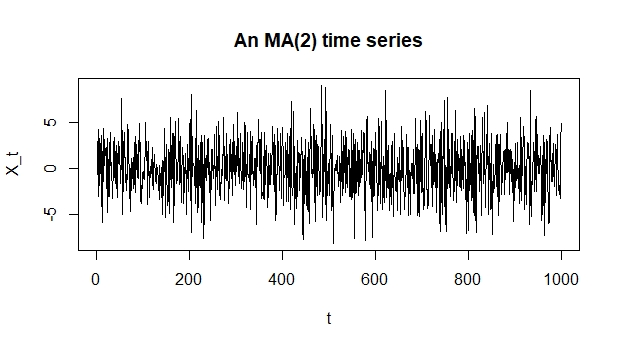
\includegraphics[width=10cm,height=5cm]{p23a.jpeg}
  %\caption{}
\end{figure}
Comments:\\
a) The mean is 0, namely $\mathbb{E}[X_t]$ in this case. The time series is stationary.\\
b) Most of the $X_t$ values are between -2.83 and 2.83, namely $\mathbb{E}[X_t]\pm{STD[X_t]}$ in this case.\\
c) The process has slight smoothed fluctuations.
\vspace{3mm}

\item
R codes:
\lstinputlisting{p24a.R}
R outputs:
\begin{figure}[H]
  \centering
  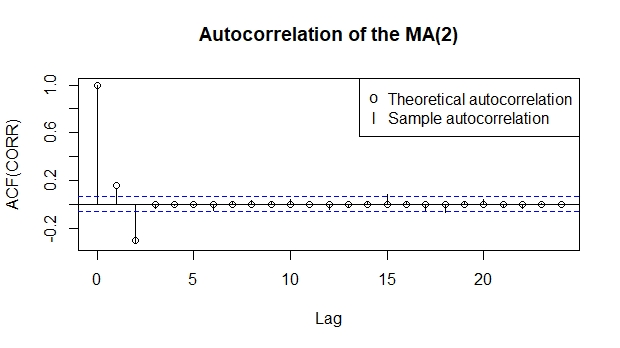
\includegraphics[width=10cm,height=5cm]{p24a.jpeg}
  %\caption{}
\end{figure}
Comments:\\
a) The theoretical autocorrelation and the sample autocorrelation are very close but still different.\\
b) When the lag is greater than 2, the sample autocorrelation is not 0 and varies.\\
c) When the lag increases to 100, the difference still exists and hardly gets small.\\
Reasons:\\
a) For this MA(2) process, we expect to see 0 autocorrelation after lag 2.\\
b) For the difference between the two types of autocorrelation, the sample length (size) 1000 is not large enough, according to the large sample theory.\\
c) For the difference, the different data sets used also matter.\\
d) For the difference, there is bias in the autocorrelation calculation and plotting in R.\footnote{ National Institute of Standards and Technology. (n.d.). \textit{Autocorrelation plot}. Retrieved from \url{https://www.itl.nist.gov/div898/handbook/eda/section3/autocopl.htm}.}

\end{enumerate}
\vspace{3mm}

\begin{prob}
\end{prob}
\begin{proof}
When a time series is weakly stationary, all observations have the same finite variance.\\
We have the variance of $X_t$
\begin{align*}
VAR[X_t]&=VAR[W_t+\theta(W_{t-1}+W_{t-2}+...)]\\
&=VAR[W_t]+\theta^2VAR[W_{t-1}]+\theta^2VAR[W_{t-2}]+...,\\ % Comment: this is infinite
&\;\textrm{since}\;COV[W_t, W_{t-|h|}]=0\\
&=\sigma^2_W+\theta^2\sum^t_{i=1}\sigma^2_W. % Comment: so this must be infinite
\end{align*}
The variance of an observation depends on t, so all the observations do not have the same variance.\\
Also,
\begin{align*}
\lim_{t\to\infty}VAR[X_t]=\infty.
\end{align*}
Hence, an MA($\infty$) process is not stationary.
\end{proof}
\begin{proof}
(Bonus) When a time series is weakly stationary, the covariance between two observations depends only on the distance h and does not depend on t.\\
We have the covariance of $X_t$ and $X_{t+|h|}$,
\begin{align*}
COV[X_t,X_{t+|h|}]&=\frac{VAR[X_t+X_{t+|h|}]+VAR[X_t]+VAR[X_{t+|h|}]}{2}\\
&=\frac{2VAR[X_t]+2VAR[X_{t+|h|}]}{2}\\
&=VAR[X_t]+VAR[X_{t+|h|}].
\end{align*}
Use the previous proof,
\begin{align*}
COV[X_t,X_{t+|h|}]&=VAR[X_t]+VAR[X_{t+|h|}]\\
&=\sigma^2_W+\theta^2\sum^t_{i=1}\sigma^2_W+\sigma^2_W+\theta^2\sum^{t+|h|}_{i=1}\sigma^2_W\\
&=2\sigma^2_W+2\theta^2\sum^t_{i=1}\sigma^2_W+\theta^2\sum^{t+|h|}_{i=t+1}\sigma^2_W.
\end{align*}
The covariance between any two observations depends on t and h. Hence, an MA($\infty$) process is not stationary.
\end{proof}
\begin{proof}
Straightforwardly,
\begin{align*}
Y_t&=X_t-X_{t-1}\\
&=W_t+\theta(W_{t-1}+W_{t-2}+...)-W_{t-1}-\theta(W_{t-2}+W_{t-3}+...)\\
&=W_t-W_{t-1}+{\theta}W_{t-1}\\
&=W_t+(\theta-1)W_{t-1}.
\end{align*}
An MA(1) process has the general equation $X_t=W_t+{\theta'}W_{t-1}$.\footnote{ Shumway, R. H., \& Stoffer, D. S. (2017). \textit{Time series analysis and its applications: with R examples}. Springer, 84.} $Y_t$ is in this form where $\theta'=\theta-1$ and is an MA(1) process.\\
To show the stationarity,
\begin{align*}
\mathbb{E}[Y_t]&=\mathbb{E}[W_t+(\theta-1)W_{t-1}]\\
&=0;\\
VAR[Y_t]&=VAR[W_t+(\theta-1)W_{t-1}]\\
&=(\theta^2-2\theta+2)\sigma^2_W;\\
COV[Y_t,Y_{t+|h|}]&=\left\{\begin{array}{ll}(\theta^2-2\theta+2)\sigma^2_W,\;\textrm{if}\;h=0,\\
\theta-1,\;\textrm{if}\;h=1,\\
0,\;\textrm{if}\;h>1.\end{array}\right.
\end{align*}
Hence, all the observations have the same finite mean and variance and the covariance between any two observations depends only on the distance h. This MA(1) process is stationary.
\end{proof}
The autocorrelation function is
\begin{align*}
\rho(h)&=\left\{\begin{array}{ll}1,\textrm{if}\;h=0,\\
\frac{1-\theta}{\theta^2-2\theta+2},\;\textrm{if}\;|h|=1,\\
0,\;\textrm{if}\;|h|>1.\end{array}\right.
\end{align*}
\vspace{3mm}

\begin{prob}
\end{prob}
\begin{enumerate}[1)]
\vspace{3mm}

\item
The backshift operator representation of this AR(2) model is given by
\begin{align*}
X_t-0X_{t-1}-(-0.8)X_{t-2}&=W_t\\
(1-0B-(-0.8)B^2)X_t&=W_t\\
(1+0.8B^2)X_t&=W_t\\
X_t&=\frac{1}{1+0.8B^2}W_t
\end{align*}
where $BX_t=X_{t-1}$ gives a concise notation of
\begin{align*}
\phi(B)X_t&=W_t\\
X_t&=\psi(B)W_t,\;\textrm{where}\;\psi(B)=\frac{1}{\phi(B)}.
\end{align*}
The autoregressive operator of this AR(2) model is
\begin{align*}
\phi(B)=1+0.8B^2.
\end{align*}
\vspace{3mm}

\item
Using the stationarity, we have the mean,
\begin{align*}
\mathbb{E}[X_t]&=\mathbb{E}[-0.8X_{t-2}+W_t]\\
\mathbb{E}[X_t]&=-0.8\mathbb{E}[X_{t-2}]+\mathbb{E}[W_t]\\
\mathbb{E}[X_t]&=-0.8\mathbb{E}[X_t]+0\\
\mathbb{E}[X_t]&=0,
\end{align*}
and the variance,
\begin{align*}
VAR[X_t]&=VAR[-0.8X_{t-2}+W_t]\\
VAR[X_t]&=0.64VAR[X_{t-2}]+VAR[W_t]\\
VAR[X_t]&=0.64VAR[X_t]+\sigma^2_W\\
VAR[X_t]&=\frac{25}{9}\sigma^2_W.
\end{align*}
\vspace{3mm}

\item
Using the results from the previous assignments ($\gamma(h)=\mathbb{E}[(X_t-\mu)(X_{t-|h|}-\mu)]$ and $\rho(h)=\frac{\gamma(h)}{\gamma(0)}$) and the reference\footnote{ Tanizaki, H. (2014). \textit{Model analysis 1}. Retrieved from \url{http://www2.econ.osaka-u.ac.jp/~tanizaki/class/2014/model_analysis1/08.pdf}.}, we have the autocovariance function, % Comment: you need to derive this
\begin{align*}
\gamma(h)&=\left\{\begin{array}{ll}VAR[X_t]=\frac{25}{9}\sigma^2_W,\textrm{if}\;h=0,\\
\frac{0}{1+0.8}\gamma(0)=0,\;\textrm{if}\;|h|=1,\\
0\gamma(1)-0.8\gamma(0)=-\frac{20}{9}\sigma^2_W,\;\textrm{if}\;|h|=2,\\
0,\;\textrm{if}\;|h|=3,\\
\frac{16}{9}\sigma^2_W,\;\textrm{if}\;|h|=4,\\
%0,\;\textrm{if}\;|h|=5,\\
%-\frac{64}{45}\sigma^2_W,\;\textrm{if}\;|h|=6,\\
%0,\;\textrm{if}\;|h|=7,\\
%\frac{256}{225}\sigma^2_W,\;\textrm{if}\;|h|=8,\\
%0,\;\textrm{if}\;|h|=9,\\
%-\frac{1024}{1125}\sigma^2_W,\;\textrm{if}\;|h|=10,\\
-0.8\gamma(h-2),\;\textrm{if}\;|h|>4.\end{array}\right.
\end{align*}
and the autocorrelation function,
\begin{align*}
\rho(h)&=\left\{\begin{array}{ll}\frac{\frac{25}{9}\sigma^2_W}{\frac{25}{9}\sigma^2_W}=1,\textrm{if}\;h=0,\\
\frac{0}{\frac{25}{9}\sigma^2_W}=0,\;\textrm{if}\;|h|=1,\\
\frac{-\frac{20}{9}\sigma^2_W}{\frac{25}{9}\sigma^2_W}=-0.8,\;\textrm{if}\;|h|=2,\\
0,\;\textrm{if}\;|h|=3,\\
0.64,\;\textrm{if}\;|h|=4,\\
%0,\;\textrm{if}\;|h|=5,\\
%-0.512,\;\textrm{if}\;|h|=6,\\
%0,\;\textrm{if}\;|h|=7,\\
%0.4096,\;\textrm{if}\;|h|=8,\\
%0,\;\textrm{if}\;|h|=9,\\
%-0.32768,\;\textrm{if}\;|h|=10,\\
\frac{-0.8\gamma(h-2)}{\frac{25}{9}}=-\frac{36}{125}\gamma(h-2),\;\textrm{if}\;|h|>4.\end{array}\right.
\end{align*}
\vspace{3mm}

\item
In this case, $\mu=0$ and $\sigma_W=2$.\\
R codes:
\lstinputlisting{p43a.R}
R outputs:
\begin{figure}[H]
  \centering
  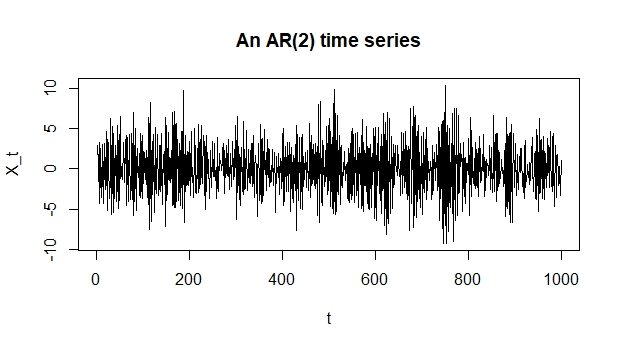
\includegraphics[width=10cm,height=5cm]{p43a.jpeg}
  %\caption{}
\end{figure}
Comments:\\
a) The mean is 0, namely $\mathbb{E}[X_t]$ in this case. The time series is stationary.\\
b) Most of the $X_t$ values are between -3.33 and 3.33, namely $\mathbb{E}[X_t]\pm{STD[X_t]}$ in this case.\\
c) The AR(2) process is almost smooth and more smooth than the previous MA(2) process.
\vspace{3mm}

\item
R codes:
\lstinputlisting{p44a.R}
R outputs:
\begin{figure}[H]
  \centering
  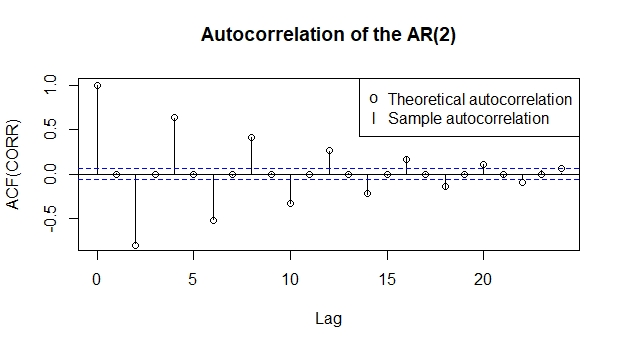
\includegraphics[width=10cm,height=5cm]{p44a.jpeg}
  %\caption{}
\end{figure}
Comments:\\
a) When the lag is even, the theoretical autocorrelation and the sample autocorrelation are very close but still different.\\
b) When the lag is odd, the sample autocorrelation is not 0 though the theoretical autocorrelation is 0.\\
c) When the lag increases to 100, the difference still exists and even gets big around some lags; especially, when the lag is 64, the difference between the two types of autocorrelation is locally maximized.\\
Reasons:\\
a) For this AR(2) process, we expect to get a geometric decay in its autocorrelation and the process (and its corresponding autocorrelation) tends to switch between positive and negative values.\footnote{ Lab8. (2019). Unpublished manuscript.}\\
b) For the difference between the two types of autocorrelation, the sample length (size) 1000 is not large enough, according to the large sample theory.\\
c) For the difference, the different data sets used also matter.\\
d) For the difference, there is bias in the autocorrelation calculation and plotting in R.\footnote{ National Institute of Standards and Technology. (n.d.). \textit{Autocorrelation plot}. Retrieved from \url{https://www.itl.nist.gov/div898/handbook/eda/section3/autocopl.htm}.}

\end{enumerate}

\end{document}
